\documentclass[a4paper,11pt]{report}
\usepackage[T1]{fontenc}
\usepackage[utf8]{inputenc}
\usepackage{lmodern}
\usepackage{graphicx}
\usepackage[margin=1in]{geometry}
\title{WildLife}
\author{Leander Maben}

\begin{document}

\maketitle
\tableofcontents

\begin{abstract}
This article talks about wildlife.
The aim is to explore latex features.
\end{abstract}

\section{Introduction}
Wildlife traditionally refers to undomesticated animal species, but has come to include all organisms that groow or live wild in an area without being introduced by humans.Wildlife can be found in all ecosystems. Deserts, forests, rainforests, plains, grasslands, and other areas, including the most developed urban areas, all have distinct forms of wildlife See \ref{tiger}. While the term in popular culture usually refers to animals that are untouched by human factors, most scientists agree that much wildlife is affected by human activities.
\begin{figure}[h]
\label{tiger}
\caption{Tiger}
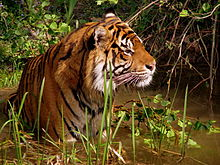
\includegraphics[width=\textwidth,keepaspectratio=true,height=\textheight]
{tiger.jpg}
\end{figure}
Humans have historically tended to separate civilization from wildlife in a number of ways, including the legal, social, and moral senses. Some animals, however, have adapted to suburban environments. This includes such animals as domesticated cats, dogs, mice, and gerbils. Some religions declare certain animals to be sacred, and in modern times, concern for the natural environment has provoked activists to protest against the exploitation of wildlife for human benefit or entertainment.

The global wildlife population decreased by 52% between 1970 and 2014, according to a World Wildlife Fund report
\section{Tourism}
Many nations have established their tourism sector around their natural wildlife. South Africa has, for example, many opportunities for tourists to see the country's wildlife in its national parks, such as the Kruger Park. In South India, the Periar Wildlife Sanctuary, Bandipur National Park and Mudumalai Wildlife Sanctuary are situated around and in forests. India is home to many national parks and wildlife sanctuaries showing the diversity of its wildlife, much of its unique fauna, and excels in the range. There are 89 national parks, 13 bio reserves and more than 400 wildlife sanctuaries across India which are the best places to go to see Bengal tigers, Asiatic lions, Indian elephants, Indian rhinoceroses, birds, and other wildlife which reflect the importance that the country places on nature and wildlife conservation.

\section{Destruction}
This subsection focuses on anthropogenic forms of wildlife destruction. The loss of animals from ecological communities is also known as defaunation.

Exploitation of wild populations has been a characteristic of modern man since our exodus from Africa 130,000 – 70,000 years ago. The rate of extinctions of entire species of plants and animals across the planet has been so high in the last few hundred years it is widely believed that we are in the sixth great extinction event on this planet; the Holocene Mass Extinction.

Destruction of wildlife does not always lead to an extinction of the species in question, however, the dramatic loss of entire species across Earth dominates any review of wildlife destruction as extinction is the level of damage to a wild population from which there is no return.[clarification needed]

The four most general reasons that lead to destruction of wildlife include overkill, habitat destruction and fragmentation, impact of introduced species and chains of extinction.
\subsection{Overkill}
Overkill happens whenever hunting occurs at rates greater than the reproductive capacity of the population is being exploited. The effects of this are often noticed much more dramatically in slow growing populations such as many larger species of fish. Initially when a portion of a wild population is hunted, an increased availability of resources (food, etc.) is experienced increasing growth and reproduction as density dependent inhibition is lowered. Hunting, fishing and so on, has lowered the competition between members of a population. However, if this hunting continues at rate greater than the rate at which new members of the population can reach breeding age and produce more young, the population will begin to decrease in numbers.

Populations that are confined to islands, whether literal islands or just areas of habitat that are effectively an "island" for the species concerned, have also been observed to be at greater risk of dramatic population rise of deaths declines following unsustainable hunting. 
\subsection{Habitat Destruction}
The habitat of any given species is considered its preferred area or territory. Many processes associated with human habitation of an area cause loss of this area and decrease the carrying capacity of the land for that species. In many cases these changes in land use cause a patchy break-up of the wild landscape. Agricultural land frequently displays this type of extremely fragmented, or relictual, habitat. Farms sprawl across the landscape with patches of uncleared woodland or forest dotted in-between occasional paddocks.

Examples of habitat destruction include grazing of bushland by farmed animals, changes to natural fire regimes, forest clearing for timber production and wetland draining for city expansion. 
\subsection{Extinction}
This final group is one of secondary effects. All wild populations of living things have many complex intertwining links with other living things around them. Large herbivorous animals such as the hippopotamus have populations of insectivorous birds that feed off the many parasitic insects that grow on the hippo. Should the hippo die out, so too will these groups of birds, leading to further destruction as other species dependent on the birds are affected. Also referred to as a domino effect, this series of chain reactions is by far the most destructive process that can occur in any ecological community.

Another example is the black drongos and the cattle egrets found in India. These birds feed on insects on the back of cattle, which helps to keep them disease-free. Destroying the nesting habitats of these birds would cause a decrease in the cattle population because of the spread of insect-borne diseases. 
Animals are conserved in several ways.One of them is through Biosphere reserves.See table \ref{bio} 
\begin{table}[h]
\centering
\label{bio}
\scalebox{1.5}{
\begin{tabular}{|c|c|c|}
\hline
Reserve & Place & Important Animal\\ \hline
Kaziranga National Park& 	Assam &	One-horned rhino\\ \hline
Gir National Park &	Gujarat &	Asiatic lions\\ \hline
Bandipur &	Karnataka 	&Tiger, Elephant\\ \hline
Dachigam &	J and K &	Hangul\\ \hline
Kanha &	M.P &	Tiger\\ \hline
Periyar &	Kerala &	Tiger, elephant\\ \hline
Ranthambore National Park &	Rajasthan &	Tiger\\ \hline 
  
\end{tabular}
}
\end{table}
\end{document}
